% Options for packages loaded elsewhere
\PassOptionsToPackage{unicode}{hyperref}
\PassOptionsToPackage{hyphens}{url}
\PassOptionsToPackage{dvipsnames,svgnames,x11names}{xcolor}
%
\documentclass[
  12pt,
  letterpaper,
  DIV=11,
  numbers=noendperiod]{scrartcl}

\usepackage{amsmath,amssymb}
\usepackage{iftex}
\ifPDFTeX
  \usepackage[T1]{fontenc}
  \usepackage[utf8]{inputenc}
  \usepackage{textcomp} % provide euro and other symbols
\else % if luatex or xetex
  \usepackage{unicode-math}
  \defaultfontfeatures{Scale=MatchLowercase}
  \defaultfontfeatures[\rmfamily]{Ligatures=TeX,Scale=1}
\fi
\usepackage{lmodern}
\ifPDFTeX\else  
    % xetex/luatex font selection
\fi
% Use upquote if available, for straight quotes in verbatim environments
\IfFileExists{upquote.sty}{\usepackage{upquote}}{}
\IfFileExists{microtype.sty}{% use microtype if available
  \usepackage[]{microtype}
  \UseMicrotypeSet[protrusion]{basicmath} % disable protrusion for tt fonts
}{}
\makeatletter
\@ifundefined{KOMAClassName}{% if non-KOMA class
  \IfFileExists{parskip.sty}{%
    \usepackage{parskip}
  }{% else
    \setlength{\parindent}{0pt}
    \setlength{\parskip}{6pt plus 2pt minus 1pt}}
}{% if KOMA class
  \KOMAoptions{parskip=half}}
\makeatother
\usepackage{xcolor}
\usepackage[margin=1in]{geometry}
\setlength{\emergencystretch}{3em} % prevent overfull lines
\setcounter{secnumdepth}{-\maxdimen} % remove section numbering
% Make \paragraph and \subparagraph free-standing
\ifx\paragraph\undefined\else
  \let\oldparagraph\paragraph
  \renewcommand{\paragraph}[1]{\oldparagraph{#1}\mbox{}}
\fi
\ifx\subparagraph\undefined\else
  \let\oldsubparagraph\subparagraph
  \renewcommand{\subparagraph}[1]{\oldsubparagraph{#1}\mbox{}}
\fi


\providecommand{\tightlist}{%
  \setlength{\itemsep}{0pt}\setlength{\parskip}{0pt}}\usepackage{longtable,booktabs,array}
\usepackage{calc} % for calculating minipage widths
% Correct order of tables after \paragraph or \subparagraph
\usepackage{etoolbox}
\makeatletter
\patchcmd\longtable{\par}{\if@noskipsec\mbox{}\fi\par}{}{}
\makeatother
% Allow footnotes in longtable head/foot
\IfFileExists{footnotehyper.sty}{\usepackage{footnotehyper}}{\usepackage{footnote}}
\makesavenoteenv{longtable}
\usepackage{graphicx}
\makeatletter
\def\maxwidth{\ifdim\Gin@nat@width>\linewidth\linewidth\else\Gin@nat@width\fi}
\def\maxheight{\ifdim\Gin@nat@height>\textheight\textheight\else\Gin@nat@height\fi}
\makeatother
% Scale images if necessary, so that they will not overflow the page
% margins by default, and it is still possible to overwrite the defaults
% using explicit options in \includegraphics[width, height, ...]{}
\setkeys{Gin}{width=\maxwidth,height=\maxheight,keepaspectratio}
% Set default figure placement to htbp
\makeatletter
\def\fps@figure{htbp}
\makeatother
\newlength{\cslhangindent}
\setlength{\cslhangindent}{1.5em}
\newlength{\csllabelwidth}
\setlength{\csllabelwidth}{3em}
\newlength{\cslentryspacingunit} % times entry-spacing
\setlength{\cslentryspacingunit}{\parskip}
\newenvironment{CSLReferences}[2] % #1 hanging-ident, #2 entry spacing
 {% don't indent paragraphs
  \setlength{\parindent}{0pt}
  % turn on hanging indent if param 1 is 1
  \ifodd #1
  \let\oldpar\par
  \def\par{\hangindent=\cslhangindent\oldpar}
  \fi
  % set entry spacing
  \setlength{\parskip}{#2\cslentryspacingunit}
 }%
 {}
\usepackage{calc}
\newcommand{\CSLBlock}[1]{#1\hfill\break}
\newcommand{\CSLLeftMargin}[1]{\parbox[t]{\csllabelwidth}{#1}}
\newcommand{\CSLRightInline}[1]{\parbox[t]{\linewidth - \csllabelwidth}{#1}\break}
\newcommand{\CSLIndent}[1]{\hspace{\cslhangindent}#1}

\usepackage{booktabs}
\usepackage{longtable}
\usepackage{array}
\usepackage{multirow}
\usepackage{wrapfig}
\usepackage{float}
\usepackage{colortbl}
\usepackage{pdflscape}
\usepackage{tabu}
\usepackage{threeparttable}
\usepackage{threeparttablex}
\usepackage[normalem]{ulem}
\usepackage{makecell}
\usepackage{xcolor}
\usepackage[default]{sourcesanspro}
\usepackage{sourcecodepro}
\usepackage{lineno}
\linenumbers
\linespread{1.2}
\KOMAoption{captions}{tableheading}
\makeatletter
\makeatother
\makeatletter
\makeatother
\makeatletter
\@ifpackageloaded{caption}{}{\usepackage{caption}}
\AtBeginDocument{%
\ifdefined\contentsname
  \renewcommand*\contentsname{Table of contents}
\else
  \newcommand\contentsname{Table of contents}
\fi
\ifdefined\listfigurename
  \renewcommand*\listfigurename{List of Figures}
\else
  \newcommand\listfigurename{List of Figures}
\fi
\ifdefined\listtablename
  \renewcommand*\listtablename{List of Tables}
\else
  \newcommand\listtablename{List of Tables}
\fi
\ifdefined\figurename
  \renewcommand*\figurename{Fig.}
\else
  \newcommand\figurename{Fig.}
\fi
\ifdefined\tablename
  \renewcommand*\tablename{Table}
\else
  \newcommand\tablename{Table}
\fi
}
\@ifpackageloaded{float}{}{\usepackage{float}}
\floatstyle{ruled}
\@ifundefined{c@chapter}{\newfloat{codelisting}{h}{lop}}{\newfloat{codelisting}{h}{lop}[chapter]}
\floatname{codelisting}{Listing}
\newcommand*\listoflistings{\listof{codelisting}{List of Listings}}
\makeatother
\makeatletter
\@ifpackageloaded{caption}{}{\usepackage{caption}}
\@ifpackageloaded{subcaption}{}{\usepackage{subcaption}}
\makeatother
\makeatletter
\@ifpackageloaded{tcolorbox}{}{\usepackage[skins,breakable]{tcolorbox}}
\makeatother
\makeatletter
\@ifundefined{shadecolor}{\definecolor{shadecolor}{rgb}{.97, .97, .97}}
\makeatother
\makeatletter
\makeatother
\makeatletter
\makeatother
\ifLuaTeX
  \usepackage{selnolig}  % disable illegal ligatures
\fi
\IfFileExists{bookmark.sty}{\usepackage{bookmark}}{\usepackage{hyperref}}
\IfFileExists{xurl.sty}{\usepackage{xurl}}{} % add URL line breaks if available
\urlstyle{same} % disable monospaced font for URLs
\hypersetup{
  colorlinks=true,
  linkcolor={blue},
  filecolor={Maroon},
  citecolor={Blue},
  urlcolor={Blue},
  pdfcreator={LaTeX via pandoc}}

\author{}
\date{}

\begin{document}
\ifdefined\Shaded\renewenvironment{Shaded}{\begin{tcolorbox}[boxrule=0pt, sharp corners, enhanced, frame hidden, breakable, interior hidden, borderline west={3pt}{0pt}{shadecolor}]}{\end{tcolorbox}}\fi

\newpage

\textbf{Impacts of artificial light at night on understory}

\[ \]

Cong Zhou\textsuperscript{1,2}, Akihiro Nakamura\textsuperscript{1},
Masatoshi Katabuchi\textsuperscript{1},

\[ \]

\textsuperscript{1} CAS Key Laboratory of Tropical Forest Ecology,
Xishuangbanna Tropical Botanical Garden, Chinese Academy of Sciences,
Menglun, Yunnan 666303, China

\textsuperscript{2} University of Chinese Academy of Sciences, Beijing
100049, China

\[ \]

\textbf{Corresponding Authors}:

Masatoshi Katabuchi

E-mail: mattocci27@gmail.com

\[ \]

\textbf{Running title}:

\newpage

\hypertarget{abstract}{%
\section{ABSTRACT}\label{abstract}}

Artificial light at night (ALAN) demonstrated a new ecological factor
that influences organisms through multi-approach. As yet, assessing the
impacts of artificial light at night on understory plants has little
attention. We evaluated whether ALAN would affect the LMA (leaf mass per
area) of understory plants through a two-year field light experiment in
tropical rubber plant forests in south China. We assumed ALAN would
affect the understory by directly increasing light supplement
aboveground and indirectly attracting insects, then changing soil
nutrients underground. Two species were chosen in this study
\emph{Colocasia gigantea (Blume) Hook. f.} representing shade species
and \emph{Melastoma candidum D. Don} representing sun species. Canopy
openness, LMA value, soil nutrients and individual distance away from
ALAN were measured. We found a negative relationship between LMA values
of the understory and the effects of ALAN, which was significant to
species \emph{Colocasia gigantea (Blume) Hook. f.} while non-significant
to species \emph{Melastoma candidum D. Don}. Results suggest that ALAN
might trigger comprehensive effects on understory.

\textbf{KEY WORDS} leaf mass per area (LMA), understory, Artificial
light at night (ALAN), \emph{Colocasia gigantea (Blume) Hook. f.} ,
\emph{Melastoma candidum D. Don}

\hypertarget{introduction}{%
\section{INTRODUCTION}\label{introduction}}

Artificial light at night (ALAN), a leading contributor to light
pollution, has disrupted ecological processes since the early 20th
century (\protect\hyperlink{ref-Longcore2004}{Longcore and Rich 2004},
\protect\hyperlink{ref-Gaston2013}{Gaston et al. 2013},
\protect\hyperlink{ref-Bennie2016}{Bennie et al. 2016}). A recent study
estimated that around 23\% of the world's inhabited land surfaces,
accounting for over 80\% of the global population, are subject to the
adverse effects of light pollution
(\protect\hyperlink{ref-Falchi2016}{2016}). Although the intensity of
ALAN varies several orders of magnitude from faint skyglow reflected
from distant cities to direct illumination of urban and suburban
vegetation (\protect\hyperlink{ref-Bennie2016}{Bennie et al. 2016}),
ALAN could influence the behaviour or physiology of broad ranges of
taxonomic groups, including mammals, birds, reptiles, amphibians,
fishes, invertebrates, and plants. It could alter ecosystem functions
{[}@ Rich2006{]}. For example, ALAN attracts insects interfering in
movement, foraging, reproduction, and development, as an important
bringer to driving insect population decline
(\protect\hyperlink{ref-Owens2020}{Owens et al. 2020},
\protect\hyperlink{ref-Boyes2021}{Boyes et al. 2021}). Many studies have
focused on how ALAN changes the behaviour of animals
(\protect\hyperlink{ref-Russart2018}{Russart and Nelson 2018}). However,
only a handful of studies have been published on the effect of ALAN on
plants (\protect\hyperlink{ref-Bennie2016}{Bennie et al. 2016},
\protect\hyperlink{ref-Speisser2021a}{Speißer et al. 2021},
\protect\hyperlink{ref-Liu2022}{\textbf{Liu2022?}}). Speißer et al.
(\protect\hyperlink{ref-Speisser2021a}{2021}) conducted plant growth
experiments with and without weak ALAN (28 lx: within the range of light
intensities at ground level under street lights) and showed that ALAN
increases the biomass of herbaceous plants. Their results suggest that
even weak ALAN acts as a light resource for plant growth. However, few
studies have examined the effects of ALAN on plant functional traits in
conditions close to their natural environment.

ALAN might, directly and indirectly, affect plant leaf functional
traits. First, ALAN might directly affect plant leaf functional traits
because ALAN could work as a light resource. Although LMA is driven by
inherent genetic mechanisms (\protect\hyperlink{ref-Asner2011}{Asner et
al. 2011}), environmental stresses (temperature, water and light) also
shape LMA. Plants can sense light through photoreceptors, allowing them
to respond to four parameters of their light environment: light spectral
quality, light intensity, light direction, and light duration
(\protect\hyperlink{ref-Rich2006}{Rich and Longcore 2006},
\protect\hyperlink{ref-Paik2019}{Paik and Huq 2019}). Terashima et al.
(\protect\hyperlink{ref-Terashima2006}{2006}) showed that the
light-saturated rate of leaf photosynthesis per unit area (\(P_{max}\))
is highly correlated with leaf structural parameters such as leaf
thickness, leaf mass per area, mesophyll surface area(\(S_{mes}\)), and
chloroplast surface area (\(S_c\)), and sun leaves are thicker than
shade leaves as the height of the palisade tissue in sun leaves is
greater than that in shade leaves. For individual species, LMA was
proportional with species distributions along the insolation gradient
and was significantly higher in evergreen versus deciduous species
(\protect\hyperlink{ref-Ackerly2002}{Ackerly et al. 2002},
\protect\hyperlink{ref-Niinemets2004}{Niinemets et al. 2004},
\protect\hyperlink{ref-Onoda2008}{Onoda et al. 2008}). Moreover, among a
local community, Ackerly et al.
(\protect\hyperlink{ref-Ackerly2002}{2002}) demonstrated that the
average values of LMA significantly increased with increasing potential
diurnal insolation (PDI).

On the other hand, ALAN might indirectly affect plant leaf functional
traits because ALAN has the potential to change soil environmental
conditions by attracting insects. Many insects orient themselves by
maintaining a constant angle to light rays and are attracted by light
{[}positive phototaxis? yes (\protect\hyperlink{ref-Baker1978}{Baker and
Sadovy 1978}, \protect\hyperlink{ref-Sotthibandhu1979}{Sotthibandhu and
Baker 1979}){]}. Previous studies showed that 30--40\% of insects die
soon after approaching street lamps for collision, overheating,
dehydration, or predation (\protect\hyperlink{ref-Minnaar2015}{Minnaar
et al. 2015}, \protect\hyperlink{ref-Owens2018}{Owens and Lewis 2018}).
Since nitrogen (N) and phosphorus (P) are the nutrients most frequently
limiting primary productivity in forest ecosystems
(\protect\hyperlink{ref-Wright2019}{Wright 2019}), dead insects killed
by ALAN could be important nutrient input for soil nutrients
(\protect\hyperlink{ref-Behie2013}{Behie and Bidochka 2013}). Soil
resources, especially N and P availability, are known to affect leaf
mass per area (LAM) and leaf N and P contents
(\protect\hyperlink{ref-Wright2004}{Wright et al. 2004},
\protect\hyperlink{ref-Riva2016}{Riva et al. 2016}), and those effects
are known to be opposite to the effects of light
(\protect\hyperlink{ref-Ackerly2002}{Ackerly et al. 2002},
\protect\hyperlink{ref-Hernandez-Vargas2019}{Hernández-Vargas et al.
2019}) (i.e., while strong light increases LMA but high levels of N
availability decrease LMA).

Here, we investigated the relationship between LMA values of the
understory and the effects of ALAN through a two-year experiment in a
tropical rubber plant forest in south China. We selected two species as
subjects of this experiment, each representing sun and shade species, to
discern differences in their responses to ALAN. Our hypothesis proposes
that ALAN would influence the understory via two distinct pathways: one
directly, as a supplementary light source for the aboveground portions
of plants, and the other indirectly, improving soil nutrient
availability for the belowground parts. Based on our hypothesis, we
anticipate two key outcomes: (a) an increase in the influence of ALAN
would correspond with a decrease in the LMA value of the understory, and
(b) the extent of canopy openness and its interaction with ALAN would
have a minor impact on the results of this experiment.

\hypertarget{materials-and-methods}{%
\section{MATERIALS AND METHODS}\label{materials-and-methods}}

\emph{Experimental setup}

ALAN field experiments were located within the Xishuangbanna Tropical
Botanical Garden (XTBG), China, in a rubber tree forest (N21°54'
E101°16') where we set 5 plots and selected two plots for this
experiment after field investigation. LED lights (10w) were used to
create an artificial light environment in all plots at night (Fig. 1).
The LED system included six components. A metal box with an opening
served as a rainproof protector. This box was attached to a tree around
1.2m from the ground. A rechargeable lithium battery (12v/30Ah) and an
electric timer controlled the timing and duration of the LED operation
at night. An electric wire connected the battery and LED, hanging from a
tree branch with a lampshade approximately 2 m from the ground. The LED
system was programmed to function automatically from 8 pm to 5 am daily.
The experiment was set up in November 2019, and leaf disc samples were
collected two years later, in November 2021.

\emph{Species Selection}

Considering the understory conditions (mature individuals and
distribution of individuals) and species specificity (it should be
evergreen species and not be the nitrogen fix plants like
\emph{Leguminosae}) of each plot, finally two species respectively in
two plots were chosen for our study, \emph{Colocasia gigantea (Blume)
Hook. f.} representing shade species and \emph{Melastoma candidum D.
Don} for sun species.

\emph{Measurements}

We measured the horizontal distance and geographic orientation of each
individual away from the LED using a tape measure representing the
relative effects of ALAN. The canopy openness of each individual was on
behalf of individual daylight interception, which was photographed by
Nikon COOLPIX4500 with a fish-eye lens (Nikon FC-e8) and then measured
using R package \emph{LeafArea}
(\protect\hyperlink{ref-Katabuchi2015}{Katabuchi 2015}). For leaf mass
per area (LMA), we used leaf disc (10mm\^{}2) punched from leaf avoiding
vein and leaf margin instead of whole-leaf to calculate individual mean
LMA value (\protect\hyperlink{ref-Maenpuen2022}{Maenpuen et al. 2022}).
We chose five healthy leaves, then five leaf discs, each leaf on species
\emph{Melastoma candidum D. Don}, and round five leaves, then seven leaf
discs on species \emph{Colocasia gigantea (Blume) Hook. f.}.

For soil nutrients (N, C, P), we collected surface soil samples (0-10 cm
depths) in five plots in June 2019 and June 2022. We took three
replicates at the place under ALAN and 10m away from ALAN separately
from each plot. After sampling, the soils were air-dried at room
temperature for one week, then sieved through 0.85mm and 0.15mm mesh
finally used for total N, C measurements by combustion using an
elemental analyzer (Vario MAX CN, Elementar Analysensysteme GmbH
(Germany)) and total P measurement by inductively coupled plasma
atomic-emission spectrometer (iCAP7400, Thermo Fisher Scientific U.S.A).
Then we calculated the relative percentage change of each nutrient
between the value in 2019 and 2022 to compare the soil nutrient change
with ALAN's effect (sampled under ALAN) and without ALAN's effect
(sampled 10m away from ALAN).

\[
X_{2022}/X_{2019}, \ \ \ (X = C,N,P)
\]

\emph{Data Analysis}

To analyze the effects of ALAN, daylight's effect, and their interaction
on both \emph{Melastoma candidum D. Don} and \emph{Colocasia gigantea
(Blume) Hook. f.}, we fitted a Bayesian linear mixed-effets model for
each species implemented in Stan
(\protect\hyperlink{ref-Carpenter2017}{Carpenter et al. 2017}). The Stan
code used to fit the models is available from Github at
https://github.com/Congon/light\_project. Leaf mass per area (LMA) of
each leaf of each individual was the response variable. Distance from
the ALAN of each individual was transformed by log and reciprocal
because the accumulation of insects and the intensity of ALAN fade away
from distance nonlinearly. We conducted individual as a random effect
for each species on our model because individuals of the same species
were non-independent. All statistical analyses were conducted in R
version 4.1.2 (\protect\hyperlink{ref-RCoreTeam2022}{R Core Team 2022}).

\hypertarget{results}{%
\section{RESULTS}\label{results}}

The effects of ALAN and daylight were significant for species
\emph{Colocasia gigantea (Blume) Hook. f.}, while species
\emph{Melastoma candidum D. Don} showed no significance. Artificial
light at night drove the averaged individual LMA value decrease for
species \emph{Colocasia gigantea (Blume) Hook. f.} (Table 1, slope:
-0.1043 {[}95\% CI: -0.1458, -0.0621{]}), and for species
\emph{Melastoma candidum D. Don} (Table 1, slope: -0.0422) although not
significant. Both species showed no significance on the interaction of
the effects of ALAN and daylight (Table 1). Loss of soil nutrients
(\(X_{2022}/X_{2019} < 1,\ (X = C,N,P)\)) were observed in general among
five plots from 2019 to 2022. The relative percentage change of each
soil nutrient showed clear difference between the place under ALAN
(\(C_{2022}/C_{2019} = 0.919\), \(N_{2022}/N_{2019} = 0.948\),
\(P_{2022}/P_{2019} = 0.537\)) and the place 10m away from ALAN
(\(C_{2022}/C_{2019} = 0.663\), \(N_{2022}/N_{2019} = 0.695\),
\(P_{2022}/P_{2019} = 0.492\)) at the plot where \emph{Colocasia
gigantea (Blume) Hook. f.} disturbed, while showed not too much
difference for the other species.

\hypertarget{discussion}{%
\section{DISCUSSION}\label{discussion}}

Although it had been demonstrated that LMA increase with insolation
(\protect\hyperlink{ref-Ackerly2002}{Ackerly et al. 2002},
\protect\hyperlink{ref-Niinemets2004}{Niinemets et al. 2004}), our
research showed the effects of night artificial light to plants should
be considered as a comprehensive situation. Artificial light at night
would exert an influence on the physiological processes of understory by
multi-approach both aboveground and undergound. For aboveground part,
artificial light at night change the light environments of plants
including light duration, light intensity and light spectral quality.
For underground part, artificial light at night might indirectly change
soil nutrients conditions by attracting insects especially as an
important nitrogen supplementary. In this study, the LMA value of
understory showed a negative relationship with the composite effects of
artificial light at night, thereinto the relationship between LMA and
soil nutrients was consistent with previous studies. Nevertheless we
could not confirm the difference in the soil nutrients was due to
artificial light at night, for soil nutrents were lost througthout
rubber plant forest because of precipitation, terrain and rubber tapping
although artificial light at night to some extent retarded the loss of
soil nutrients in our experiment place. Furthermore the results of
understory response could vary according to the species specificity (sun
species showed no significance in our study) and artificial light
resource (varying intensities of artificial light could cause different
results (\protect\hyperlink{ref-Bennie2016}{Bennie et al. 2016})).

There was research showed that plants' biomass would increase under
artificial light through controlling experiment
(\protect\hyperlink{ref-Speisser2021a}{Speißer et al. 2021}), but our
study showed the allocation of the changing part of biomass could be
channelled into mixed results. Controlling experiment probably tend to
underestimate the species interaction and unpredictable environmental
heterogeneity caused by natural and artificial factors, because many
irreplaceable features of field conditions, such as subtle nutrients
change, herbivores and competitors are usually absent. Thus, adequate
tests of the influence of artificial light at night on understory will
entail more experimental work under field conditions. In future work,
diverse artificial light resource in light spectral quality and light
intensity and more understory group will be needed to simulate
comprehensive effcts of artificial light from plant physiology to plant
community. In conclusion, the general pattern how understory species
responds to artificial light at night remains unknown. Our study showed
the LMA value of some understory species would decrease with artificial
light at night. This negative effect could indicate that increments of
artificial light at night might bring about a physiological suppression
to those understory plants with which applied implications for
environmental management and urban ecological planning.

\hypertarget{ackonwledgements}{%
\section{ACKONWLEDGEMENTS}\label{ackonwledgements}}

\hypertarget{literature-cited}{%
\section{LITERATURE CITED}\label{literature-cited}}

\hypertarget{refs}{}
\begin{CSLReferences}{1}{0}
\leavevmode\vadjust pre{\hypertarget{ref-Ackerly2002}{}}%
Ackerly, D., C. Knight, S. Weiss, K. Barton, and K. Starmer. 2002.
\href{https://doi.org/10.1007/s004420100805}{Leaf size, specific leaf
area and microhabitat distribution of chaparral woody plants:
Contrasting patterns in species level and community level analyses}.
Oecologia 130:449--457.

\leavevmode\vadjust pre{\hypertarget{ref-Asner2011}{}}%
Asner, G. P., R. E. Martin, R. Tupayachi, R. Emerson, P. Martinez, F.
Sinca, G. V. N. Powell, S. J. Wright, and A. E. Lugo. 2011.
\href{https://doi.org/10.1890/09-1999.1}{Taxonomy and remote sensing of
leaf mass per area ({LMA}) in humid tropical forests}. Ecological
Applications 21:85--98.

\leavevmode\vadjust pre{\hypertarget{ref-Baker1978}{}}%
Baker, R. R., and Y. Sadovy. 1978.
\href{https://doi.org/10.1038/276818a0}{The distance and nature of the
light-trap response of moths}. Nature 276:818--821.

\leavevmode\vadjust pre{\hypertarget{ref-Behie2013}{}}%
Behie, S. W., and M. J. Bidochka. 2013.
\href{https://doi.org/10.3390/insects4030413}{Insects as a {Nitrogen
Source} for {Plants}}. Insects 4:413--424.

\leavevmode\vadjust pre{\hypertarget{ref-Bennie2016}{}}%
Bennie, J., T. W. Davies, D. Cruse, and K. J. Gaston. 2016.
\href{https://doi.org/10.1111/1365-2745.12551}{Ecological effects of
artificial light at night on wild plants}. Journal of Ecology
104:611--620.

\leavevmode\vadjust pre{\hypertarget{ref-Boyes2021}{}}%
Boyes, D. H., D. M. Evans, R. Fox, M. S. Parsons, and M. J. O. Pocock.
2021. \href{https://doi.org/10.1126/sciadv.abi8322}{Street lighting has
detrimental impacts on local insect populations}. Science Advances
7:eabi8322.

\leavevmode\vadjust pre{\hypertarget{ref-Carpenter2017}{}}%
Carpenter, B., A. Gelman, M. D. Hoffman, D. Lee, B. Goodrich, M.
Betancourt, M. Brubaker, J. Guo, P. Li, and A. Riddell. 2017.
\href{https://doi.org/10.18637/jss.v076.i01}{Stan: {A Probabilistic
Programming Language}}. Journal of Statistical Software 76:1--32.

\leavevmode\vadjust pre{\hypertarget{ref-Falchi2016}{}}%
Falchi. 2016. \href{https://doi.org/10.1126/sciadv.1600377}{The new
world atlas of artificial night sky brightness}.
https://www.science.org/doi/10.1126/sciadv.1600377.

\leavevmode\vadjust pre{\hypertarget{ref-Gaston2013}{}}%
Gaston, K. J., J. Bennie, T. W. Davies, and J. Hopkins. 2013.
\href{https://doi.org/10.1111/brv.12036}{The ecological impacts of
nighttime light pollution: A mechanistic appraisal}. Biological Reviews
88:912--927.

\leavevmode\vadjust pre{\hypertarget{ref-Hernandez-Vargas2019}{}}%
Hernández-Vargas, G., L. R. Sánchez-Velásquez, J. C. López-Acosta, J. C.
Noa-Carrazana, and Y. Perroni. 2019.
\href{https://doi.org/10.1111/1440-1703.1267}{Relationship between soil
properties and leaf functional traits in early secondary succession of
tropical montane cloud forest}. Ecological Research 34:213--224.

\leavevmode\vadjust pre{\hypertarget{ref-Katabuchi2015}{}}%
Katabuchi, M. 2015.
\href{https://doi.org/10.1007/s11284-015-1307-x}{{LeafArea}: An {R}
package for rapid digital image analysis of leaf area}. Ecological
Research 30:1073--1077.

\leavevmode\vadjust pre{\hypertarget{ref-Longcore2004}{}}%
Longcore, T., and C. Rich. 2004.
\href{https://doi.org/10.1890/1540-9295(2004)002\%5B0191:ELP\%5D2.0.CO;2}{Ecological
light pollution}. Frontiers in Ecology and the Environment 2:191--198.

\leavevmode\vadjust pre{\hypertarget{ref-Maenpuen2022}{}}%
Maenpuen, P., M. Katabuchi, Y. Onoda, C. Zhou, J.-L. Zhang, and Y.-J.
Chen. 2022. \href{https://doi.org/10.1002/ajb2.16038}{Sources and
consequences of mismatch between leaf disc and whole-leaf leaf mass per
area ({LMA})}. American Journal of Botany 109:1242--1250.

\leavevmode\vadjust pre{\hypertarget{ref-Minnaar2015}{}}%
Minnaar, C., J. G. Boyles, I. A. Minnaar, C. L. Sole, and A. E.
McKechnie. 2015. \href{https://doi.org/10.1111/1365-2664.12381}{Stacking
the odds: Light pollution may shift the balance in an ancient
predator\textendash prey arms race}. Journal of Applied Ecology
52:522--531.

\leavevmode\vadjust pre{\hypertarget{ref-Niinemets2004}{}}%
Niinemets, Ü., O. Kull, and J. D. Tenhunen. 2004.
\href{https://doi.org/10.1111/j.1365-3040.2003.01143.x}{Within-canopy
variation in the rate of development of photosynthetic capacity is
proportional to integrated quantum flux density in temperate deciduous
trees}. Plant, Cell \& Environment 27:293--313.

\leavevmode\vadjust pre{\hypertarget{ref-Onoda2008}{}}%
Onoda, Y., F. Schieving, and N. P. R. Anten. 2008.
\href{https://doi.org/10.1093/aob/mcn013}{Effects of {Light} and
{Nutrient Availability} on {Leaf Mechanical Properties} of {Plantago}
major: {A Conceptual Approach}}. Annals of Botany 101:727--736.

\leavevmode\vadjust pre{\hypertarget{ref-Owens2020}{}}%
Owens, A. C. S., P. Cochard, J. Durrant, B. Farnworth, E. K. Perkin, and
B. Seymoure. 2020.
\href{https://doi.org/10.1016/j.biocon.2019.108259}{Light pollution is a
driver of insect declines}. Biological Conservation 241:108259.

\leavevmode\vadjust pre{\hypertarget{ref-Owens2018}{}}%
Owens, A. C. S., and S. M. Lewis. 2018.
\href{https://doi.org/10.1002/ece3.4557}{The impact of artificial light
at night on nocturnal insects: {A} review and synthesis}. Ecology and
Evolution 8:11337--11358.

\leavevmode\vadjust pre{\hypertarget{ref-Paik2019}{}}%
Paik, I., and E. Huq. 2019.
\href{https://doi.org/10.1016/j.semcdb.2019.03.007}{Plant
photoreceptors: {Multi-functional} sensory proteins and their signaling
networks}. Seminars in Cell \& Developmental Biology 92:114--121.

\leavevmode\vadjust pre{\hypertarget{ref-RCoreTeam2022}{}}%
R Core Team. 2022. R: {A} language and environment for statistical
computing. Manual, {R Foundation for Statistical Computing}, {Vienna,
Austria}.

\leavevmode\vadjust pre{\hypertarget{ref-Rich2006}{}}%
Rich, C., and T. Longcore. 2006. Ecological consequences of artificial
night lighting.

\leavevmode\vadjust pre{\hypertarget{ref-Riva2016}{}}%
Riva, E. G. de la, M. Olmo, H. Poorter, J. L. Ubera, and R. Villar.
2016. \href{https://doi.org/10.1371/journal.pone.0148788}{Leaf {Mass}
per {Area} ({LMA}) and {Its Relationship} with {Leaf Structure} and
{Anatomy} in 34 {Mediterranean Woody Species} along a {Water
Availability Gradient}}. PLOS ONE 11:e0148788.

\leavevmode\vadjust pre{\hypertarget{ref-Russart2018}{}}%
Russart, K. L. G., and R. J. Nelson. 2018.
\href{https://doi.org/10.1002/jez.2173}{Artificial light at night alters
behavior in laboratory and wild animals}. Journal of Experimental
Zoology Part A: Ecological and Integrative Physiology 329:401--408.

\leavevmode\vadjust pre{\hypertarget{ref-Sotthibandhu1979}{}}%
Sotthibandhu, S., and R. R. Baker. 1979.
\href{https://doi.org/10.1016/0003-3472(79)90015-0}{Celestial
orientation by the large yellow underwing moth, {Noctua} pronuba {L}}.
Animal Behaviour 27:786--800.

\leavevmode\vadjust pre{\hypertarget{ref-Speisser2021a}{}}%
Speißer, B., Y. Liu, and M. van Kleunen. 2021.
\href{https://doi.org/10.1111/1365-2745.13607}{Biomass responses of
widely and less-widely naturalized alien plants to artificial light at
night}. Journal of Ecology 109:1819--1827.

\leavevmode\vadjust pre{\hypertarget{ref-Terashima2006}{}}%
Terashima, I., Y. T. Hanba, Y. Tazoe, P. Vyas, and S. Yano. 2006.
\href{https://doi.org/10.1093/jxb/erj014}{Irradiance and phenotype:
Comparative eco-development of sun and shade leaves in relation to
photosynthetic {CO2} diffusion}. Journal of Experimental Botany
57:343--354.

\leavevmode\vadjust pre{\hypertarget{ref-Wright2004}{}}%
Wright, I. J., P. B. Reich, M. Westoby, D. D. Ackerly, Z. Baruch, F.
Bongers, J. Cavender-Bares, T. Chapin, J. H. C. Cornelissen, M. Diemer,
J. Flexas, E. Garnier, P. K. Groom, J. Gulias, K. Hikosaka, B. B.
Lamont, T. Lee, W. Lee, C. Lusk, J. J. Midgley, M.-L. Navas, Ü.
Niinemets, J. Oleksyn, N. Osada, H. Poorter, P. Poot, L. Prior, V. I.
Pyankov, C. Roumet, S. C. Thomas, M. G. Tjoelker, E. J. Veneklaas, and
R. Villar. 2004. \href{https://doi.org/10.1038/nature02403}{The
worldwide leaf economics spectrum}. Nature 428:821--827.

\leavevmode\vadjust pre{\hypertarget{ref-Wright2019}{}}%
Wright, S. J. 2019. \href{https://doi.org/10.1002/ecm.1382}{Plant
responses to nutrient addition experiments conducted in tropical
forests}. Ecological Monographs 89:e01382.

\end{CSLReferences}

\newpage

\textbf{Fig. 1.} The distribution of individuals around the ALAN and the
illustration of the experiment setup. The distribution of individuals
LMA values around the artificial light of two experimental species (A
and C). Photographs of the experimental plots during the day and night
(B and D).

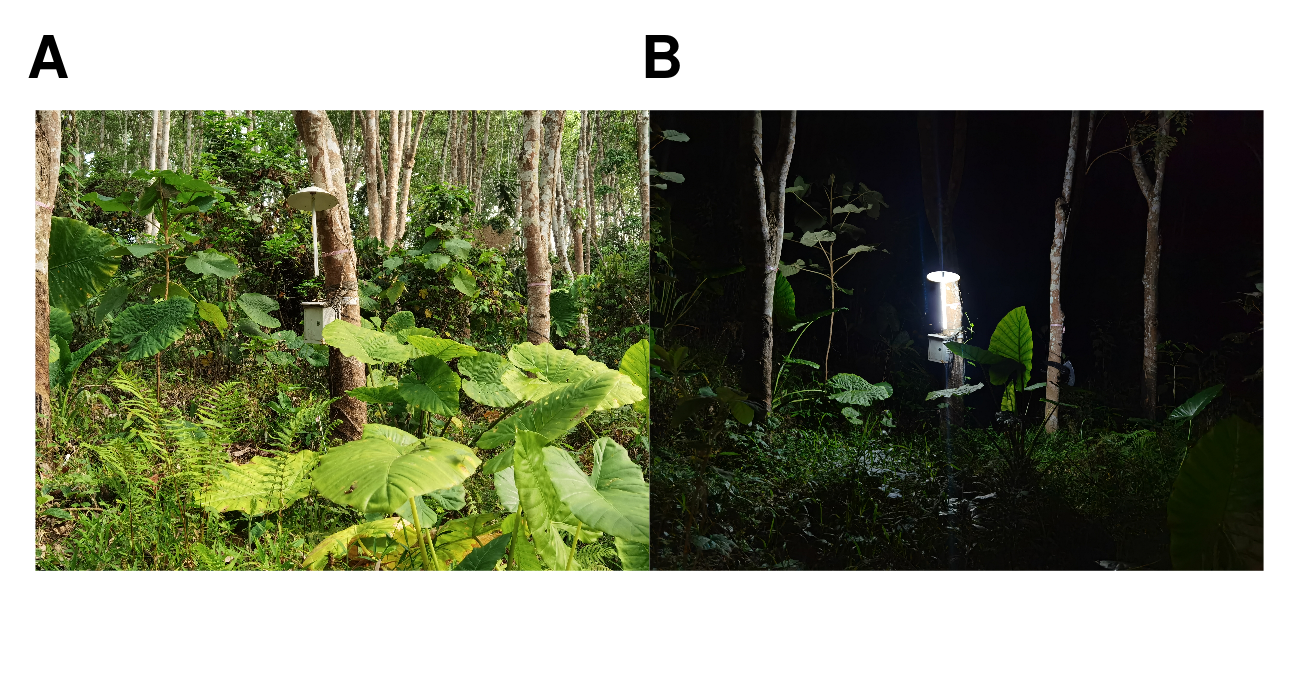
\includegraphics{../figs/merge.png}

\newpage

\begin{table}

\caption{Coefficients table}
\centering
\begin{tabular}[t]{r|l|r|>{}l}
\hline
X & Parameters & mean\_value & quantile\_interval\\
\hline
\multicolumn{4}{l}{\textbf{Melastoma\_candidum}}\\
\hline
\hspace{1em}1 & ALAN's effect & -0.0422 & [-0.1129, 0.0276]\\
\hline
\hspace{1em}2 & Daylight's effect & -0.0006 & [-0.0761, 0.0744]\\
\hline
\hspace{1em}3 & interaction & -0.0308 & [-0.0836, 0.0216]\\
\hline
\multicolumn{4}{l}{\textbf{Colocasia\_gigantea}}\\
\hline
\hspace{1em}4 & ALAN's effect & -0.1043 & \textbf{[-0.1458, -0.0621]}\\
\hline
\hspace{1em}5 & Daylight's effect & 0.0495 & \textbf{[0.0051, 0.0938]}\\
\hline
\hspace{1em}6 & interaction & -0.0120 & [-0.0428, 0.0195]\\
\hline
\end{tabular}
\end{table}

\textbf{Table. 1.} Results of Bayesian general linear mixed-effect
models testing the effects of artificial light at night, daylight and
interaction on experimental species. Significant effects (p \textless{}
0.05) are in bold.

\newpage



\end{document}
